% !TEX TS-program = pdflatex
% !TEX encoding = UTF-8 Unicode

% This is a simple template for a LaTeX document using the "article" class.
% See "book", "report", "letter" for other types of document.

\documentclass[11pt]{article} % use larger type; default would be 10pt

\usepackage[utf8]{inputenc} % set input encoding (not needed with XeLaTeX)

%%% Examples of Article customizations
% These packages are optional, depending whether you want the features they provide.
% See the LaTeX Companion or other references for full information.

%%% PAGE DIMENSIONS
\usepackage{geometry} % to change the page dimensions
\geometry{a4paper} % or letterpaper (US) or a5paper or....
% \geometry{margin=2in} % for example, change the margins to 2 inches all round
% \geometry{landscape} % set up the page for landscape
%   read geometry.pdf for detailed page layout information

\usepackage{graphicx} % support the \includegraphics command and options

% \usepackage[parfill]{parskip} % Activate to begin paragraphs with an empty line rather than an indent

%%% PACKAGES
\usepackage{booktabs} % for much better looking tables
\usepackage{array} % for better arrays (eg matrices) in maths
\usepackage{paralist} % very flexible & customisable lists (eg. enumerate/itemize, etc.)
\usepackage{verbatim} % adds environment for commenting out blocks of text & for better verbatim
\usepackage{subfig} % make it possible to include more than one captioned figure/table in a single float
% These packages are all incorporated in the memoir class to one degree or another...

%%% HEADERS & FOOTERS
\usepackage{fancyhdr} % This should be set AFTER setting up the page geometry
\pagestyle{fancy} % options: empty , plain , fancy
\renewcommand{\headrulewidth}{0pt} % customise the layout...
\lhead{}\chead{}\rhead{}
\lfoot{}\cfoot{\thepage}\rfoot{}

%%% SECTION TITLE APPEARANCE
\usepackage{sectsty}
\allsectionsfont{\sffamily\mdseries\upshape} % (See the fntguide.pdf for font help)
% (This matches ConTeXt defaults)
\usepackage{graphicx}
\usepackage{hyperref}
\usepackage{listings}
\usepackage{color}

\definecolor{dkgreen}{rgb}{0,0.6,0}
\definecolor{gray}{rgb}{0.5,0.5,0.5}
\definecolor{mauve}{rgb}{0.58,0,0.82}

\lstset{frame=tb,
  language=Python,
  aboveskip=3mm,
  belowskip=3mm,
  showstringspaces=false,
  columns=flexible,
  basicstyle={\small\ttfamily},
  numbers=none,
  numberstyle=\tiny\color{gray},
  keywordstyle=\color{blue},
  commentstyle=\color{dkgreen},
  stringstyle=\color{mauve},
  breaklines=true,
  breakatwhitespace=false
  tabsize=3
}
%%% ToC (table of contents) APPEARANCE
\usepackage[nottoc,notlof,notlot]{tocbibind} % Put the bibliography in the ToC
\usepackage[titles,subfigure]{tocloft} % Alter the style of the Table of Contents
\renewcommand{\cftsecfont}{\rmfamily\mdseries\upshape}
\renewcommand{\cftsecpagefont}{\rmfamily\mdseries\upshape} % No bold!
\usepackage{amsmath}
%%% END Article customizations

%%% The "real" document content comes below...

\title{Project 1}
\author{Charles Loelius}
%\date{} % Activate to display a given date or no date (if empty),
         % otherwise the current date is printed 

\begin{document}
\maketitle

\section{Scattering Equations for  $n-^{10}Be $ with Arbitrary L}
\subsection{Radial Scattering Equations}
We can write Schrodinger's equations as 
\begin{equation}
H\psi=E\psi
\end{equation}

Now using a basic separation of variables and have that in spherical coordinates with azimuthal symmetry(which we have in this instance)\\

\begin{equation}
\psi=\Sigma_{l=0}^\infty (2L+1)i^LP_l(\cos\theta)\frac{1}{kr}\chi_L(r)
\end{equation}

We can then just consider the r equation, leaving us with:

\begin{equation}
(-\frac{\hbar^2}{2\mu}(\frac{d^2}{dr^2}-\frac{L(L+1)}{r^2})+V(r)-E)\chi_L(r)=0
\end{equation}

Where we can then plug in for V:\\
\begin{equation}
(-\frac{\hbar^2}{2\mu}(\frac{d^2}{dr^2}-\frac{L(L+1)}{r^2})+\frac{V_0}{1+e^{\frac{r-R_{ws}}{a_{ws}}}}-E)\chi_L(r)=0
\end{equation}

We can represent this as:\\

\begin{equation}
\boxed{\chi''(r)=\frac{2\mu}{\hbar^2}(\frac{V_0}{1+e^{\frac{r-R_{ws}}{a_{ws}}}}-E)\chi+\frac{L(L+1)}{r^2}\chi}
\end{equation}
\subsection{Scattering Boundary Conditions}
Now, if we plug in numbers for all of the constants, and make some assumptions for E and L, we are able to solve this numerically, if in addition we provide some sort of boundary conditions. We know that in order to prevent the terms from blowing up, this means that we need $\chi_L(0)=0$, which is one such condition. We also need to have, for an elastic collision, the condition that at infinity we should expect the wavefunction to return to the form $e^{ikr}$. This can be written as at some chosen distance $a$ we set the values of the equation to be 0 everywhere except at $\theta=0$, where we would want $e^{ika+\delta}$, noting tangentially that k is determined by the mass and energy of the neutron. This is explicitly:\\

\begin{equation}
k=\frac{p}{h}=\sqrt{\frac{2mE}{\hbar^2}}
\end{equation}

From this we see that for any L value, we would simply match that\\

\begin{equation}
\chi(a)=H_L^-+S_LH_L^+\approx \sin(ka-\frac{L\pi}{2}+\delta_L)
\end{equation}

\section{Plotting Radial Behaviour}

We have as follows the radial wave functions generated via the script at the end of this report:\\


\vspace{1mm}
\begin{figure}[H]
\centering
\includegraphics[width=.5\linewidth]{"chiE1L0"}
\end{figure}
\vspace{1mm}


\vspace{1mm}
\begin{figure}[H]
\centering
\includegraphics[width=.5\linewidth]{"chiE1L1"}
\end{figure}
\vspace{1mm}


\vspace{1mm}
\begin{figure}[H]
\centering
\includegraphics[width=.5\linewidth]{"chiE1L2"}
\end{figure}
\vspace{1mm}


\vspace{1mm}
\begin{figure}[H]
\centering
\includegraphics[width=.5\linewidth]{"chiE10L0"}
\end{figure}
\vspace{1mm}


\vspace{1mm}
\begin{figure}[H]
\centering
\includegraphics[width=.5\linewidth]{"chiE10L1"}
\end{figure}
\vspace{1mm}


\vspace{1mm}
\begin{figure}[H]
\centering
\includegraphics[width=.5\linewidth]{"chiE10L2"}
\end{figure}
\vspace{1mm}

\newpage
\section{Delta as Function of Energy}
We see then that from the same code we have.\\

\vspace{1mm}
\begin{figure}[H]
\centering
\includegraphics[width=.5\linewidth]{"deltavenL0"}
\end{figure}
\vspace{1mm}


\vspace{1mm}
\begin{figure}[H]
\centering
\includegraphics[width=.5\linewidth]{"deltavenL1"}
\end{figure}
\vspace{1mm}


\vspace{1mm}
\begin{figure}[H]
\centering
\includegraphics[width=.5\linewidth]{"deltavenL2"}
\end{figure}
\vspace{1mm}

\newpage
\section{Resonances}

While we can see resonances in the delta functions, most clearly in the L=2 case, we can see this even more clearly in the cross sections, once again calculated in the script attached, and which are plotted below.\\


\vspace{1mm}
\begin{figure}[H]
\centering
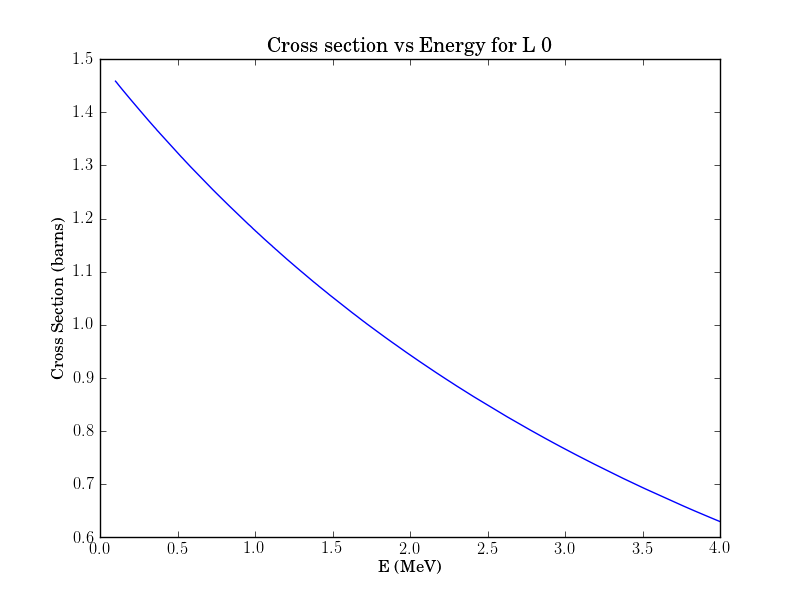
\includegraphics[width=.5\linewidth]{CrossSectionL0}
\end{figure}
\vspace{1mm}

\vspace{1mm}
\begin{figure}[H]
\centering
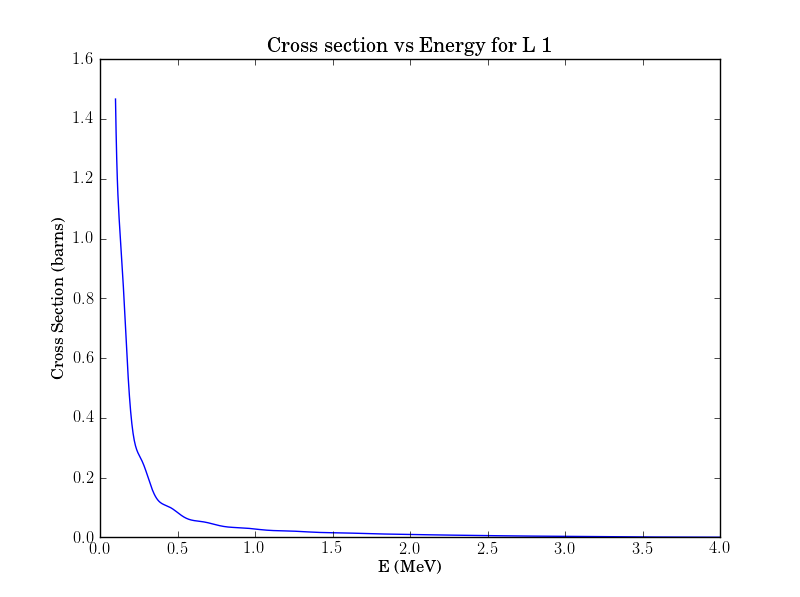
\includegraphics[width=.5\linewidth]{CrossSectionL1}
\end{figure}
\vspace{1mm}

\vspace{1mm}
\begin{figure}[H]
\centering
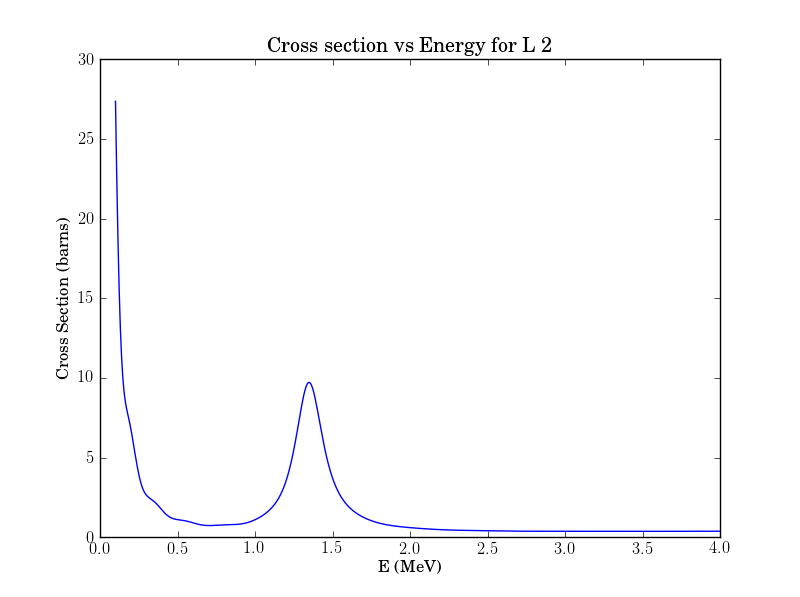
\includegraphics[width=.5\linewidth]{CrossSectionL2}
\end{figure}
\vspace{1mm}
\newpage
\section{Appendix: Code for generating graphs}
\lstinputlisting{chiscript.py}

\end{document}
